\section{Overview}\seclabel{Overview}

In this section, we informally describe our approach with a few simple example programs.

\subsection{Motivating Example}

\begin{figure}
\centering
\begin{tabular}{ccc}
\begin{lstlisting}
int sign(int x) { 
  int sgn;
  if (x < 0)
    sgn = -1
  else 
    sgn = 1
 return sgn
}
(*@ \vspace{0.1in} @*)
\end{lstlisting}
&
&
\begin{lstlisting}
int sign'(int x) {
  int sgn;
  if (x < 0)
    sgn = -1
  else if (x==0)
    sgn = 0
  else 
    sgn = 1
 return sgn
}
\end{lstlisting}
\\
\end{tabular}
\caption{Two simple implementations of the \emph{sign} operation.}
\figlabel{SignExample}
\end{figure}


Consider the simple example program of~\figref{SignExample}, inspired by an example from~\cite{RM:TOPLAS07}. For this example, we would like to establish that $sign$ and $sign'$ only differ in the case where $x=0$.

As a first naive attempt one could try to analyze each version of the program separately and compare the (abstract) results. However, this is clearly unsound, as equivalence under abstraction does not entail concrete equivalence. For example, using a interval analysis~\cite{TODO} would yield that in both programs the value of \scode{sgn} ranges in the same interval $[-1,1]$, missing the fact that $sign$ never returns the value $0$.


\paragraph{Establishing equivalence under abstraction}
To establish equivalence under abstraction, we need to abstract relationships between the values of variables in $sign$ and $sign'$. Specifically, we need to track the relationship between the values of \scode{sgn} in both versions and see whether we can establish their equivalence.

We reduce the problem of analysis across two programs to the problem of analyzing a single program by constructing a \emph{correlating program}. The correlating program represents the behaviors of both programs, and allows us to reason about relationships between variables in both.

\begin{figure}
\centering
\begin{lstlisting}
// Nimrod - please fill this 
\end{lstlisting}
\caption{Correlating program $sign \correlate sign'$.}
\figlabel{SignCorrelating}
\end{figure}


\figref{SignCorrelating} shows the correlating program for the programs of~\figref{SignExample}. Using the correlating program, we can directly track the relationship between \scode{sgn} in $sign$ and its corresponding variable \scode{sgn'} in $sign'$. Unfortunately, any domain with convex constraints will still fail to capture the precise relationship between \scode{sgn} and \scode{sgn'}. For example, using the polyhedra abstract domain~\cite{TODO}, the relationship between \scode{sgn} and \scode{sgn'} in the correlating program would be $\TODO{\langle constraint-here \rangle}$.

An obvious, but prohibitively expensive, solution to the problem is to use disjunctive completion~\cite{TODO}, moving to a powerset domain in which every abstract state is a set of convex objects (e.g., set of polyhedra). However, using such domain would significantly limit the applicability of the approach.

The desirable solution is a partially disjunctive domain, in which only certain disjunctions are kept separate during the analysis, while others are merged. The challenge in our setting is in keeping the partition fine enough such that equivalence could be preserved, without reaching exponential blowup.

\paragraph{How to partition}
We base our choice of explicit disjunctions to be kept based on their effect on variable equivalence.

\begin{figure}
\begin{tabular}{cc}
\imagetop{
\begin{tabular}{l}
\subfloat[c][$sign$]{
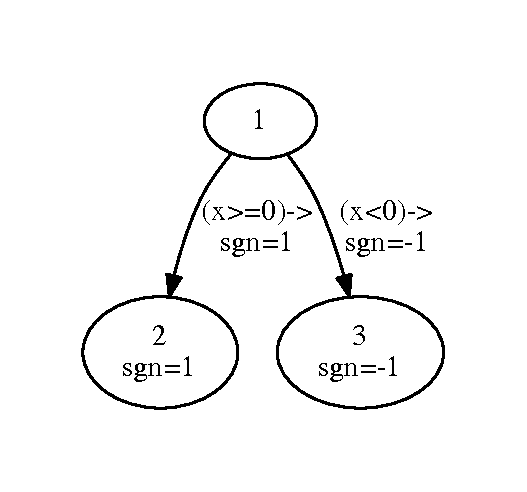
\includegraphics[width=1.2in,clip=true,trim = 20pt 20pt 30pt 20pt]{figures/sign} 
 }
 \\
 \subfloat[c][$sign'$]{
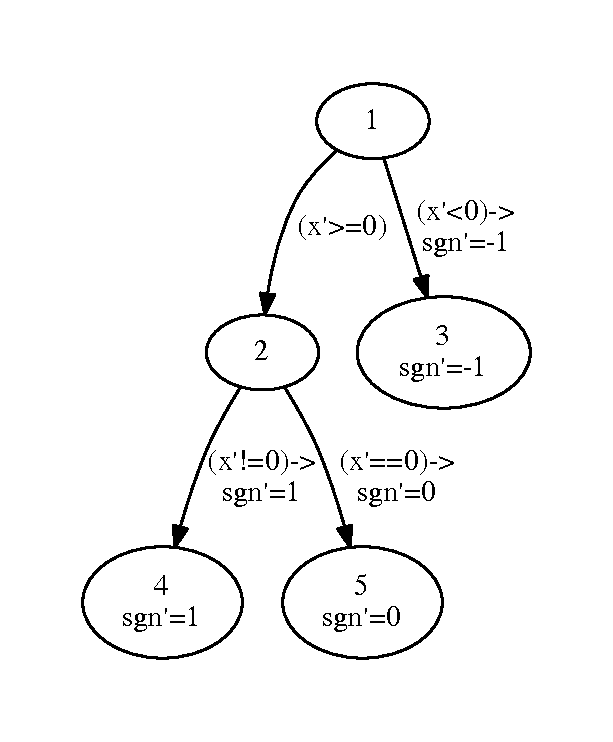
\includegraphics[width=1.2in,clip=true,trim = 20pt 20pt 30pt 20pt]{figures/sign-tag}
 }
\end{tabular}}
&
\imagetop{
\subfloat[c][$sign \correlate sign'$]{
 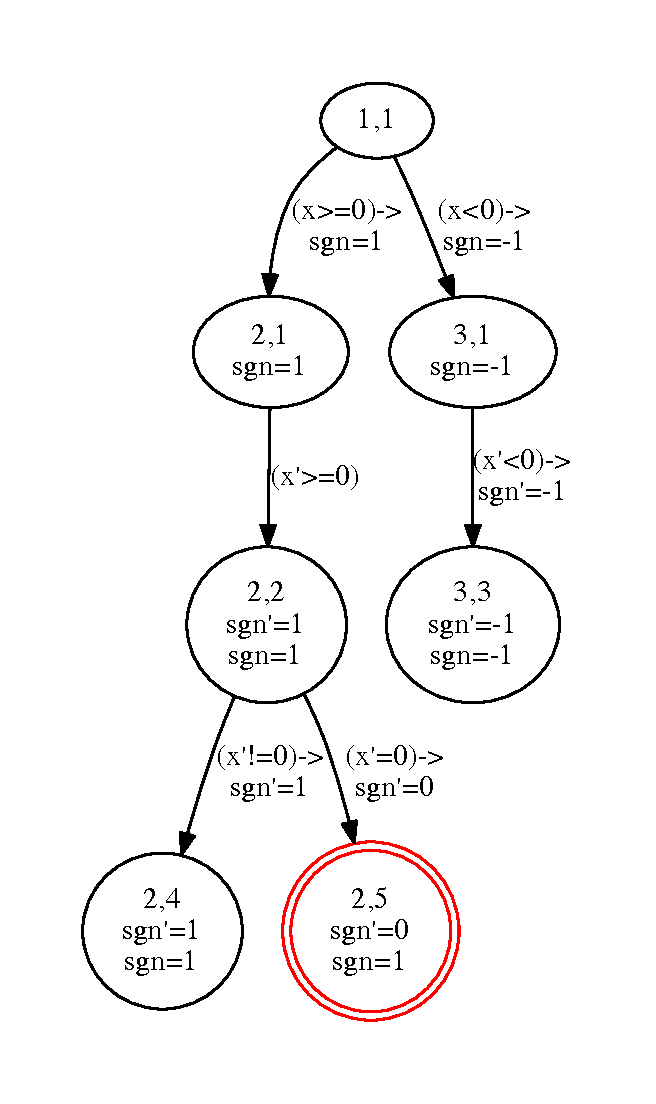
\includegraphics[width=1.4in,clip=true,trim = 20pt 20pt 30pt 20pt]{figures/sign-correlated}
 }}
\end{tabular}
\caption{Transition systems for the programs of \figref{SignExample} and \figref{SignCorrelating}.}\label{Fi:Blah}
\end{figure}


\ignore{
An alternative way to track the state across both programs is to define a correlating semantics (e.g., \cite{TODO}) where both programs are executed in lock-step and then abstract this correlating semantics.
}

\paragraph{Widening}

